\documentclass[12pt]{article}
\usepackage{fancyhdr}
\usepackage{datetime}
\usepackage{enumitem}
\usepackage{graphicx}
\graphicspath{ {images/} }
%\usepackage{showframe}

%custom variables
\newdate{date}{16}{09}{2016}
\newcommand{\hwNum}{1}
\newcommand{\assignmenttype}{Homework}


%header
\pagestyle{fancy}
\lhead{Daniel Andronov}
\chead{\thepage}
\rhead{\assignmenttype}
\cfoot{\thepage}

\fancyheadoffset[LO,RE]{1pt}
\fancyheadoffset[RO,LE]{1pt}

%titlepage
\title{\assignmenttype}
\author{Daniel Andronov}
\date{\displaydate{date}}

%addition settings
\topmargin=-0.45in
\evensidemargin=0in
\oddsidemargin=0in
\textwidth=6.5in
\textheight=9.0in
\headsep=0.25in
%start the sections from 3
\setcounter{section}{3}
\setcounter{subsection}{-1}
%enumerate left margin
\setlist[enumerate,1]{leftmargin=2.6cm}

\begin{document}
\maketitle
\newpage

\subsection{Prelab}
\begin{enumerate}[label=\textbf{Question \arabic*)}]
	\item  \begin{enumerate}[label=\alph*)]
			\item ? 
			\item T
			\item F, after each response, the connection is closed. 
			\item F, that field indicates when the packet was sent
		\end{enumerate}
	\item  \begin{enumerate}[label=\alph*)]
			\item  
			\item 
			\item 
		\end{enumerate}
	\item
	\item
	\item
\end{enumerate}

\subsection{HTTP}


\begin{enumerate}[label=\textbf{  Question \arabic*) }]
	\item abcdefg
	\item The browser is running HTTP1.1.\\ My computer's IP address is 172.16.160.130\\
	\item bc.edu's  IP address is 136.167.2.220\\
	\item The source port is 54910 and the destination port is 80.\\
	\item The source is now 80 and the destination is 54910. \\
	\item The server is running Apache.\\	The HTML file the was requested was last modified on Tuesday, October 4th 	2016 at 17:17:01 GMT.\\
	\item There were a total of 9 GET messages sent. This could be either for reduancy, so that if packets are lost, at least one will make it through the network to bc.edu in order to initiate a respone, or part of some parallelization of certain process that each send their own HTTP GET message.



\subsection{DNS}

	\item The query and response are both send via UDP.
	\item The source port is 42422 and the destination port is 53.
	\item The DNS query is sent to 172.16.160.2 and $dig$ reveals that the DNS local server IP is the same

	\begin{figure}[h]
		\caption{The result of the dig command reports the local DNS IP }
		\centering
		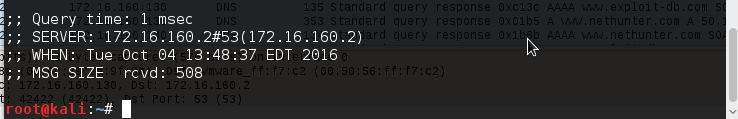
\includegraphics[scale = 0.75]{DNS_IP}
	\end{figure}

	\item

\end{enumerate}


\section{Additional Questions}
Extra Questions here

\paragraph{Additonal Question 1}
Description of the first addition Question
\end{document}
This is never printed